\documentclass{standalone}
\usepackage{tikz}
\begin{document}
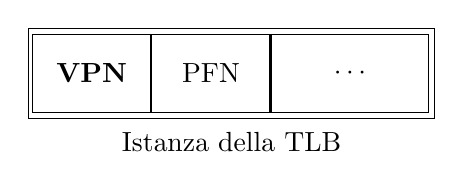
\begin{tikzpicture}
    \draw

    %% **
    % node[draw, rectangle, minimum length=1.5cm, minimum height=1cm, fill=white, anchor=180](e1){}

    (-0.05,-1)node[draw, rectangle, minimum height=1.15cm, minimum width=5.15cm, anchor=180, label={[label distance=-1.7cm]:Istanza della TLB}]{}
    (0,-1)node[draw, rectangle, minimum width=1.5cm, minimum height=1cm, fill=white, align=center, anchor=180](e0){\textbf{VPN}}
    (e0.0)node[draw, rectangle, minimum width=1.5cm, minimum height=1cm, fill=white, align=center, anchor=180](e1){PFN}
    (e1.0)node[draw, rectangle, minimum width=2cm, minimum height=1cm, fill=white, align=center, anchor=180](e2){$\cdots$}
    ;
\end{tikzpicture}
\end{document}